\documentclass[aspectratio=169,11pt]{beamer}

\usetheme{Madrid}
\usecolortheme{seahorse}

\usepackage{graphicx}
\usepackage{booktabs}
\usepackage{amsmath}
\usepackage{tikz}

\definecolor{rubinblue}{RGB}{0,73,144}
\definecolor{rubingold}{RGB}{255,199,44}

\setbeamercolor{title}{fg=rubinblue}
\setbeamercolor{frametitle}{fg=rubinblue}
\setbeamercolor{structure}{fg=rubinblue}

\title{\textbf{Primary Mirror Thermal Control}}
\subtitle{Prediction Methods and Control Algorithms for Rubin Observatory}
\author{Christopher Stubbs and Johnny Esteves\\[0.3em]
\small\textit{Analysis performed with extensive use of Claude Code}}
\date{January 2026}
\institute{Vera C. Rubin Observatory}

\begin{document}

%=============================================================================
\begin{frame}
\titlepage
\end{frame}

%=============================================================================
\begin{frame}{The Challenge}

\begin{columns}
\begin{column}{0.5\textwidth}
\textbf{At sunset, the mirror must:}
\begin{itemize}
    \item Match ambient temperature
    \item Match ambient cooling rate
    \item Preferably be slightly cold
\end{itemize}

\vspace{1em}

\textbf{Why it's hard:}
\begin{itemize}
    \item 2-hour thermal time constant
    \item Must predict 3+ hours ahead
    \item Weather is variable
\end{itemize}
\end{column}

\begin{column}{0.5\textwidth}
\centering
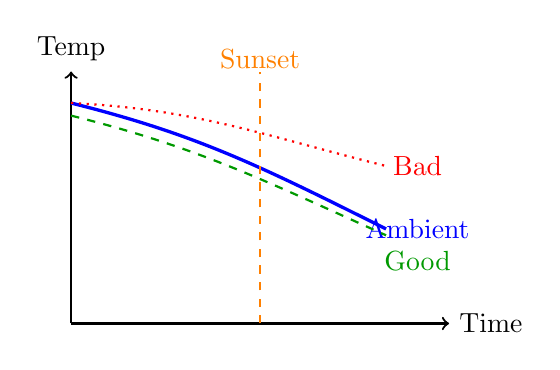
\begin{tikzpicture}[scale=0.8]
    \draw[thick,->] (0,0) -- (6,0) node[right] {Time};
    \draw[thick,->] (0,0) -- (0,4) node[above] {Temp};

    % Ambient temperature
    \draw[blue,very thick] (0,3.5) .. controls (2,3) and (3,2.5) .. (5,1.5);
    \node[blue] at (5.5,1.5) {Ambient};

    % Good mirror track
    \draw[green!60!black,thick,dashed] (0,3.3) .. controls (2,2.8) and (3,2.3) .. (5,1.4);
    \node[green!60!black] at (5.5,1) {Good};

    % Bad mirror track
    \draw[red,thick,dotted] (0,3.5) .. controls (2,3.4) and (3,3) .. (5,2.5);
    \node[red] at (5.5,2.5) {Bad};

    % Sunset line
    \draw[orange,thick,dashed] (3,0) -- (3,4);
    \node[orange] at (3,4.2) {Sunset};
\end{tikzpicture}

\small
\textit{Good control anticipates the cooling trend}
\end{column}
\end{columns}

\end{frame}

%=============================================================================
\begin{frame}{Two Key Questions}

\begin{block}{1. Prediction: What will conditions be at sunset?}
\begin{itemize}
    \item Temperature $T_\text{sunset}$: How cold will it be?
    \item Rate $\dot{T}_\text{sunset}$: How fast is it cooling?
\end{itemize}
\end{block}

\vspace{1em}

\begin{block}{2. Control: How do we get the mirror there?}
\begin{itemize}
    \item Pre-sunset: Drive to predicted conditions
    \item Overnight: Track ambient as it evolves
\end{itemize}
\end{block}

\vspace{1em}

\begin{alertblock}{Key Insight}
Matching both temperature \textbf{AND rate} at sunset dramatically improves overnight performance.
\end{alertblock}

\end{frame}

%=============================================================================
\begin{frame}{Prediction Methods Tested}

\centering
\begin{tabular}{l|cc}
\toprule
\textbf{Method} & \textbf{Type} & \textbf{Description} \\
\midrule
Ridge Regression & Traditional ML & Simple, fast, interpretable \\
\textbf{Random Forest} & Ensemble ML & Best overall performance \\
Gradient Boosting & Ensemble ML & Competitive with RF \\
LSTM Network & Deep Learning & Sequence modeling \\
Transformer & Deep Learning & Attention mechanism \\
\bottomrule
\end{tabular}

\vspace{1em}

\textbf{Features used:}
\begin{itemize}
    \item Recent temperature history (3 days)
    \item Seasonal encoding (day of year)
    \item Previous days' sunset temperatures
\end{itemize}

\end{frame}

%=============================================================================
\begin{frame}{Prediction Results: Temperature}

\centering
\includegraphics[width=0.75\textwidth]{report1_fig1_method_comparison.png}

\vspace{0.5em}

\textbf{At 3-hour lead time:}
\begin{itemize}
    \item Random Forest: \textbf{1.09°C RMS} (best)
    \item Ridge Regression: 1.07°C RMS (surprisingly competitive)
    \item Neural networks: 1.3-1.4°C RMS (worse due to limited data)
\end{itemize}

\end{frame}

%=============================================================================
\begin{frame}{LLM-Inspired Approaches: Can We Beat Random Forest?}

\begin{columns}
\begin{column}{0.45\textwidth}
\textbf{The Idea: Treat Temps as ``Text''}
\begin{enumerate}
    \item Tokenize temps into 100 bins
    \item Learn embeddings (like word vectors)
    \item Process with LSTM or Transformer
    \item Predict temperature change
\end{enumerate}

\vspace{0.5em}

\textbf{Results at 3h Lead Time:}
\begin{tabular}{l|c}
\footnotesize Method & \footnotesize RMS \\
\hline
\footnotesize \textbf{Random Forest} & \footnotesize \textbf{1.01°C} \\
\footnotesize LSTM + Embed & \footnotesize 1.31°C \\
\footnotesize Transformer & \footnotesize 1.43°C \\
\end{tabular}
\end{column}

\begin{column}{0.55\textwidth}
\centering
\includegraphics[width=\textwidth]{report1_fig2_llm_comparison.png}
\end{column}
\end{columns}

\vspace{0.3em}

\begin{alertblock}{Why RF Wins}
Limited data (385 samples), tabular structure favors trees, tokenization loses precision. LLMs might win with more data + weather forecasts.
\end{alertblock}

\end{frame}

%=============================================================================
\begin{frame}{Prediction Results: Rate of Change}

\begin{columns}
\begin{column}{0.5\textwidth}
\centering
\textbf{Rate Prediction Accuracy}

\vspace{0.5em}

\begin{tabular}{l|c}
\toprule
\textbf{Method} & \textbf{RMS (°C/h)} \\
\midrule
Ridge Regression & 0.49 \\
\textbf{Random Forest} & \textbf{0.47} \\
Gradient Boosting & 0.47 \\
\bottomrule
\end{tabular}
\end{column}

\begin{column}{0.5\textwidth}
\textbf{Key Finding:}

\vspace{0.5em}

Rate prediction error is \textbf{constant across lead times} ($\sim$0.47°C/h).

\vspace{1em}

This means:
\begin{itemize}
    \item Atmospheric variability is the limit
    \item Earlier predictions aren't worse
    \item We can confidently use 3h predictions
\end{itemize}
\end{column}
\end{columns}

\end{frame}

%=============================================================================
\begin{frame}{Prediction Recommendation}

\begin{block}{Use Random Forest for Both Predictions}
\centering
\begin{tabular}{l|cc}
\toprule
& \textbf{Temperature} & \textbf{Rate} \\
\midrule
At 3h lead & 1.09°C RMS & 0.47°C/h RMS \\
At 1h lead & 0.80°C RMS & 0.46°C/h RMS \\
\bottomrule
\end{tabular}
\end{block}

\vspace{1em}

\textbf{Why Random Forest?}
\begin{itemize}
    \item Best accuracy for both quantities
    \item Robust to missing data
    \item Fast inference ($<$10ms)
    \item Easy to retrain monthly
\end{itemize}

\end{frame}

%=============================================================================
\begin{frame}{Control Algorithm: The Key Formula}

\begin{block}{Rate-Matching Setpoint}
\Large
\[
\boxed{T_\text{setpoint} = T_\text{target} + \tau \cdot \dot{T}_\text{target} - \sigma_\text{cold}}
\]
\end{block}

\normalsize
\vspace{0.5em}

\begin{itemize}
    \item $T_\text{target}$: Target temperature (predicted or measured)
    \item $\dot{T}_\text{target}$: Target cooling rate (typically negative)
    \item $\tau = 2$ hours: Mirror thermal time constant
    \item $\sigma_\text{cold}$: Cold bias (0.2°C pre-sunset, 0.1°C overnight)
\end{itemize}

\vspace{0.5em}

\textbf{Physical meaning}: If ambient is cooling at 1°C/h, set mirror 2°C colder so it warms toward ambient at the same rate.

\vspace{0.5em}

\textbf{Critical constraint}: Setpoint rate limited to $\pm$2°C/hour to prevent thermal gradients.

\end{frame}

%=============================================================================
\begin{frame}{Control Algorithm: Dual-Setpoint Approach}

\begin{columns}
\begin{column}{0.5\textwidth}
\textbf{Pre-Sunset (dome closed)}

\vspace{0.5em}

\begin{itemize}
    \item HVAC holds interior at \textbf{FLAT} temp
    \item Mirror equilibrates naturally
    \item Apply 0.3°C cold bias
\end{itemize}

\vspace{0.5em}

$T_{HVAC} = T_{pred} - 0.3°C$ (constant)

\vspace{0.5em}

\small\textit{No tracking of exterior temp before sunset}
\end{column}

\begin{column}{0.5\textwidth}
\textbf{At Sunset}

Dome opens $\to$ interior air instantly = exterior

\vspace{0.5em}

\textbf{Overnight (dome open)}

\begin{itemize}
    \item Rate-matching control
    \item 0.3°C cold bias
\end{itemize}

\vspace{0.5em}

$T_{sp} = T_{amb} + 2h \cdot \dot{T}_{amb} - 0.3°C$
\end{column}
\end{columns}

\end{frame}

%=============================================================================
\begin{frame}{Control Results: At Sunset}

\centering
\begin{tabular}{l|cc}
\toprule
\textbf{Metric} & \textbf{Temp-Only} & \textbf{Rate-Matching} \\
\midrule
Temperature RMS & 0.80°C & \textbf{0.69°C} \\
Rate RMS & 0.87°C/h & \textbf{0.34°C/h} \\
\% Days Warm & 65\% & \textbf{40\%} \\
\bottomrule
\end{tabular}

\vspace{1em}

\begin{alertblock}{Key Result}
Rate-matching reduces rate error by \textbf{61\%} and achieves desired cold bias.
\end{alertblock}

\end{frame}

%=============================================================================
\begin{frame}{Control Results: Overnight}

\begin{columns}
\begin{column}{0.5\textwidth}
\centering
\textbf{Overnight Tracking Error}

\vspace{0.5em}

\begin{tabular}{l|c}
\toprule
\textbf{Strategy} & \textbf{RMS} \\
\midrule
Temperature-Only & 0.53°C \\
\textbf{Rate-Matching} & \textbf{0.30°C} \\
\midrule
\textit{Improvement} & \textit{44\%} \\
\bottomrule
\end{tabular}
\end{column}

\begin{column}{0.5\textwidth}
\textbf{Why it works:}

\vspace{0.5em}

Better initial conditions (matching both $T$ and $\dot{T}$) propagate through the entire night.

\vspace{1em}

\textbf{At sunset:} Mirror is already tracking the ambient trend, not fighting against it.
\end{column}
\end{columns}

\end{frame}

%=============================================================================
\begin{frame}{Cold Bias Optimization}

\begin{columns}
\begin{column}{0.45\textwidth}
\centering
\textbf{Finding the Optimal Cold Bias}

\vspace{0.5em}

\begin{tabular}{c|cc}
\toprule
\textbf{Bias} & \textbf{RMS} & \textbf{\% Warm} \\
\midrule
0.0°C & 0.33°C & 55\% \\
0.1°C & 0.34°C & 35\% \\
0.2°C & 0.38°C & 22\% \\
\textbf{0.3°C} & \textbf{0.44°C} & \textbf{15\%} \\
0.4°C & 0.51°C & 11\% \\
\bottomrule
\end{tabular}

\vspace{0.5em}

\small
\textbf{0.3°C} gives 68\% ideal range, only 15\% warm.
\end{column}

\begin{column}{0.55\textwidth}
\centering
\includegraphics[width=\textwidth]{fig76_fixed_parameter_sweep.png}
\end{column}
\end{columns}

\end{frame}

%=============================================================================
\begin{frame}{Adaptive vs Fixed Bias}

\begin{columns}
\begin{column}{0.5\textwidth}
\textbf{Should bias adapt to conditions?}

\vspace{0.5em}

Tested approaches:
\begin{itemize}
    \item Rate-adaptive: $\sigma = 0.15 + k|\dot{T}|$
    \item Uncertainty-adaptive
    \item Combined
\end{itemize}

\vspace{0.5em}

\begin{tabular}{l|cc}
\toprule
\textbf{Strategy} & \textbf{\% Warm} & \textbf{\% Ideal} \\
\midrule
Fixed 0.2°C & 17\% & \textbf{72\%} \\
\textbf{Fixed 0.3°C} & \textbf{11\%} & 70\% \\
Rate-Adaptive & 15\% & 63\% \\
\bottomrule
\end{tabular}
\end{column}

\begin{column}{0.5\textwidth}
\textbf{Conclusion:}

\vspace{0.5em}

Fixed bias wins!
\begin{itemize}
    \item Simpler to implement
    \item More robust
    \item Adaptive adds complexity without clear benefit
\end{itemize}

\vspace{0.5em}

\textbf{Recommended:} 0.3°C fixed bias
\begin{itemize}
    \item 70\% ideal range
    \item Only 11\% warm
    \item Mean offset $-0.31$°C
\end{itemize}
\end{column}
\end{columns}

\end{frame}

%=============================================================================
\begin{frame}{Dual-Setpoint Control Examples}

\centering
\includegraphics[width=0.95\textwidth]{fig75_fixed_dual_setpoint_examples.png}

\small
Before sunset: mirror (green) is FLAT at HVAC setpoint (not tracking exterior). At sunset: dome opens. Overnight: rate-matching control.

\end{frame}

%=============================================================================
\begin{frame}{Example Day Operation}

\centering
\includegraphics[width=0.85\textwidth]{fig34_example_days_overview.png}

\small
Blue: actual ambient. Orange: evolving prediction. Green dashed: setpoint. Red: mirror.

\end{frame}

%=============================================================================
\begin{frame}{Summary: Key Numbers}

\centering
\begin{tabular}{l|c}
\toprule
\textbf{Metric} & \textbf{Value} \\
\midrule
\multicolumn{2}{c}{\textit{Prediction (3h lead)}} \\
Temperature RMS & 1.09°C \\
Rate RMS & 0.47°C/h \\
\midrule
\multicolumn{2}{c}{\textit{Dual-Setpoint Control (0.3°C bias)}} \\
Overnight Tracking RMS & 0.44°C \\
Mean Offset & $-0.26$°C (cold) \\
\% Time in Ideal Range & 68\% \\
\% Time Warm & 15\% \\
\bottomrule
\end{tabular}

\end{frame}

%=============================================================================
\begin{frame}{Recommendations}

\begin{block}{1. Use Random Forest Predictions}
Train separate models for temperature and rate. Retrain monthly.
\end{block}

\begin{block}{2. Dual-Setpoint Control}
Pre-sunset: $T_{HVAC} = T_{pred} - 0.3°C$ (FLAT, constant)\\
Overnight: $T_{sp} = T_{amb} + 2h \times \dot{T}_{amb} - 0.3°C$
\end{block}

\begin{block}{3. Rate Limit Setpoint Changes}
Max $\pm 2°C$/hour to prevent thermal gradients.
\end{block}

\begin{alertblock}{Expected Outcome}
0.44°C RMS overnight. Mean $-0.26°C$ (few tenths cold). 68\% ideal. Only 15\% warm.
\end{alertblock}

\end{frame}

%=============================================================================
\begin{frame}{Questions?}

\centering
\vspace{2em}

{\Large\textbf{Thank you}}

\vspace{2em}

\textbf{Full Reports Available:}
\begin{itemize}
    \item Report 1: Prediction Methods Comparison (11 pages)
    \item Report 2: Thermal Control Algorithms (12 pages)
\end{itemize}

\vspace{2em}

\textit{Thermal Control Analysis Team}\\
\textit{January 2026}

\end{frame}

\end{document}
